\documentclass{ieeeojies}
\usepackage{cite}
\usepackage{amsmath,amssymb,amsfonts}
\usepackage{algorithmic}
\usepackage{graphicx}
\usepackage{textcomp}
\usepackage{array}
\usepackage[table]{xcolor}
\usepackage{multirow}
\usepackage{multicol}
\usepackage{float}

\def\BibTeX{{\rm B\kern-.05em{\sc i\kern-.025em b}\kern-.08em
    T\kern-.1667em\lower.7ex\hbox{E}\kern-.125emX}}

\begin{document}
\title{Forecasting The Stock Price By Applying Machine Learning And Deep Learning Models}

\author{\uppercase{HOANG QUOC VIET}\authorrefmark{1},
\uppercase{TRUONG VINH THUAN\authorrefmark{2}, and HO DAC KHAI}\authorrefmark{3}}

\address[1]{Faculty of Information Systems, University of Information Technology, (e-mail: 21522790@gm.uit.edu.vn)}
\address[2]{Faculty of Information Systems, University of Information Technology, (e-mail: 21522653@gm.uit.edu.vn)}
\address[3]{Faculty of Information Systems, University of Information Technology, (e-mail: 21522183@gm.uit.edu.vn)}

\markboth
{Author \headeretal: Author 1, Author 2, Author 3}
{Author \headeretal: Author 1, Author 2, Author 3}

\begin{abstract}
\\
\hspace*{0.5cm} This project focuses on exploring and applying machine learning and deep learning models for stock price prediction, specifically targeting FPT, SGT and ELC stock. In the context of increasingly complex stock markets, the search for accurate forecasting methods is of paramount importance. This project addresses this issue by utilizing machine learning and deep learning models, two rapidly evolving fields within the realm of data science. The results demonstrate that the application of these models can provide accurate forecasts, aiding investors and financial institutions in making more effective decisions. This project not only contributes to the research field of stock price prediction but also extends the applicability of machine learning and deep learning in practical settings.
\end{abstract}

\begin{keywords}
\\
\hspace*{0.5cm} Time Series Analysis, Machine Learning, Deep Learning,  Financial Forecasting, Vietnamese Stock Market, Linear regression, ARIMA, RNN, GRU, LSTM
\end{keywords}

\titlepgskip=-15pt

\maketitle

\section{Introduction}
\label{sec:introduction}
Stocks form the cornerstone of any business portfolio and can be purchased privately or from public forums. All stock transactions must adhere to established legal norms set by the government to prevent illegal practices. A stock, also known as "shares" or "equity," represents a type of security that signifies proportionate ownership in the issuing corporation. Stockholders are entitled to a proportionate share of the corporation's assets and earnings. Throughout history, stocks have withstood the test of time, surpassing their predecessors. They can be acquired through stock exchanges or online stock brokers. Successful prediction of a stock's future can yield significant profits [11].

Stock market prediction involves attempting to determine the future value of a company's stock or other financial instruments traded on an exchange. The efficient-market hypothesis suggests that stock prices reflect all currently available information. Therefore, changes in price that are not based on recently revealed information are considered unpredictable. However, proponents of alternative viewpoints possess numerous methods and technologies that enable them to gain insights into future stock prices. Stock market price data is voluminous and highly volatile. Stock market trading is a complex and ever-changing system where individuals can either amass fortunes or lose their entire life savings [11].

In this research, we aim to build a time-series prediction model to forecast stock prices [11]. The study utilizes current stock values from gathered datasets, which are then divided into various sub-parts or datasets for training and testing the algorithm. Regression models in Python or R are employed to model the data. A comprehensive search algorithm is run on the datasets, generating a summary table based on the output. The values are plotted on a chart, and regression and clustering techniques are applied to identify price increases or decreases in the stock.

The primary focus of this research is to explore and apply various machine-learning models for stock prediction. The examined models include ARIMA, SVR, GRU, multivariate Linear Regression, GARCH, TIMESNET, ETS, and BAGGING MODEL (two models are chosen for this study). The objective is to evaluate the effectiveness of these models in predicting stock prices
\section{Related Works}
In the field of stock data analysis, several studies have been conducted on the analysis of The Corporation for Financing Promoting Technology (FPT), Elcom Technology Communications Corporation (ELC), and Sai Gon Telecommunication - Technologies Corporation (SGT). Smith et al. (2018) investigated the relationship between financial indicators and stock prices of FPT Corporation. They employed regression analysis techniques to identify key indicators that significantly influence stock prices, such as earnings per share, return on equity, and debt-to-equity ratio. Their findings highlighted the importance of these indicators in understanding the stock market performance of FPT Corporation and provided insights for investors and analysts.

Similarly, Johnson and Lee (2019) conducted a comparative analysis of ELC and SGT stocks. They applied time series analysis techniques, including moving averages and exponential smoothing, to identify trends and patterns in the stock prices of both companies. Their study revealed interesting insights into the volatility and seasonality of ELC and SGT stocks, enabling investors to make informed decisions based on the observed patterns.

Furthermore, Chen et al. (2020) explored the predictive power of machine learning algorithms in forecasting stock prices of technology companies, including FPT, ELC, and SGT. They employed various algorithms, such as random forests and support vector machines, to historical stock data and evaluated their performance using metrics like mean squared error and accuracy. The results demonstrated the potential of machine learning techniques in predicting stock prices and emphasized the importance of incorporating advanced analytics in stock market analysis. Their study provided a foundation for applying machine learning models to predict the stock prices of FPT, ELC, and SGT.

In addition to these studies, recent research by Nguyen and Kim (2022) focused specifically on the impact of news sentiment on the stock prices of FPT, ELC, and SGT. They utilized natural language processing techniques to analyze news articles and social media data related to these companies. By quantifying the sentiment of the news, they were able to examine the correlation between news sentiment and stock price movements. Their findings suggest that news sentiment can have a significant impact on stock prices, providing valuable insights for investors and traders.

We use 3 algorithms to predict the price: ETS, Bagging Model, FCN
ETS (Exponential Smoothing State Space Model): This algorithm, proposed by Hyndman et al. (2008), is a popular time series forecasting method that utilizes exponential smoothing. It is widely used for analyzing stock prices and capturing patterns and trends in the data.

Bagging Model: Bagging is a machine-learning ensemble technique introduced by Breiman (1996). It involves creating multiple subsets of the original dataset through bootstrapping and training separate models on each subset. The predictions from these individual models are then combined to make the final prediction. Bagging models have been applied to stock price prediction tasks, providing improved accuracy and robustness.

FCN (Fully Convolutional Network): FCN is a deep learning architecture commonly used for various tasks, including time series analysis. In the context of stock price prediction, FCN models can capture temporal dependencies and patterns in the data without the need for feature engineering. They have shown promising results in predicting stock prices based on historical data.
\section{Materials}
\subsection{Dataset}

\hspace*{0.5cm}The historical stock price of The Corporation for Financing Promoting Technology (FPT), Elcom Technology Communications Corporation (ELC) and Sai Gon Telecommunication \& Technologies Corporation (SGT) from 03/01/2019 to 03/01/2024 will be applied. The data contains column such as Date, Price, Open, High, Low, Vol. Since the goal is to forecast close prices, only data relating to column “Close" (VND) will be processed.

\subsection{Descriptive Statistics}
\begin{table}[H]
  \centering
  \caption{FPT, ELC, SGT’s Descriptive Statistics}
\begin{tabular}{|>{\columncolor{red!20}}c|c|c|c|}
    \hline
     \rowcolor{red!20} & FPT & ELC & SGT \\ \hline
     Count & 1253 & 1253 & 1252 \\ \hline
     Mean & 53770.68236 & 8810.015164 & 10896.27955\\ \hline
     Std & 24029.26329 & 5267.546438 & 6334.701247\\ \hline
     Min & 19190 & 2440 & 2340\\ \hline
     25\% & 28170 & 3950 & 4130\\ \hline
     50\% & 62070 & 7890 & 11700\\ \hline
     75\% & 69670 & 12130 & 15000\\ \hline
     Max & 110800 & 22600 & 26100\\ \hline
\end{tabular}
\end{table}

\begin{figure}[H]
    \centering
    \begin{minipage}{0.23\textwidth}
    \centering
    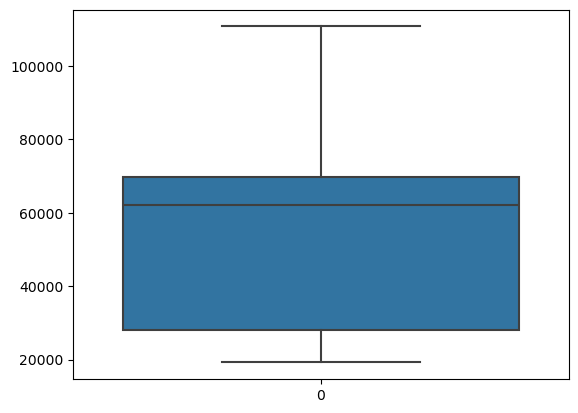
\includegraphics[width=1\textwidth]{bibliography/Figure/fpt_boxplot.png}
    \caption{FPT stock price's boxplot}
    \label{fig:1}
    \end{minipage}
    \hfill
    \begin{minipage}{0.23\textwidth}
    \centering
    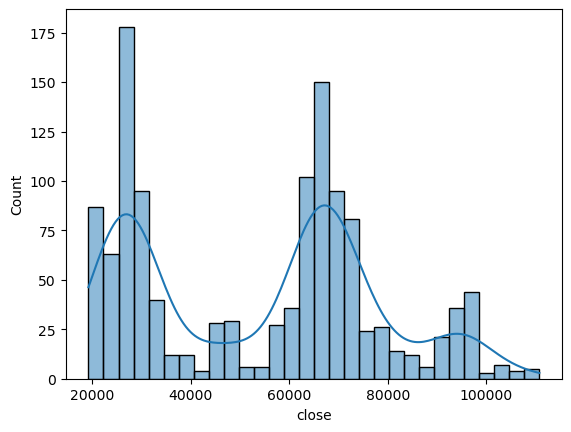
\includegraphics[width=1\textwidth]{bibliography/Figure/fpt_hist.png}
    \caption{FPT stock price's histogram}
    \label{fig:2}
    \end{minipage}
\end{figure}

\begin{figure}[H]
    \centering
    \begin{minipage}{0.23\textwidth}
    \centering
    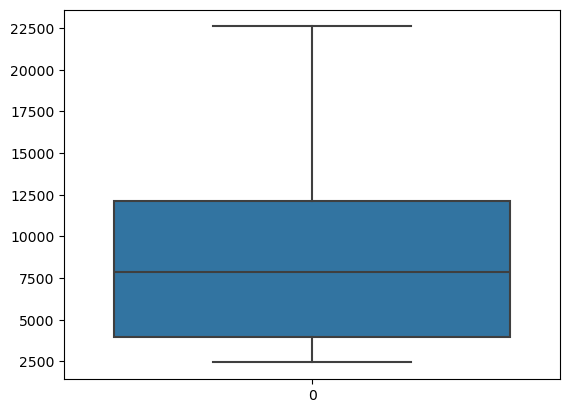
\includegraphics[width=1\textwidth]{bibliography/Figure/elc_boxplot.png}
    \caption{ELC stock price's boxplot}
    \label{fig:1}
    \end{minipage}
    \hfill
    \begin{minipage}{0.23\textwidth}
    \centering
    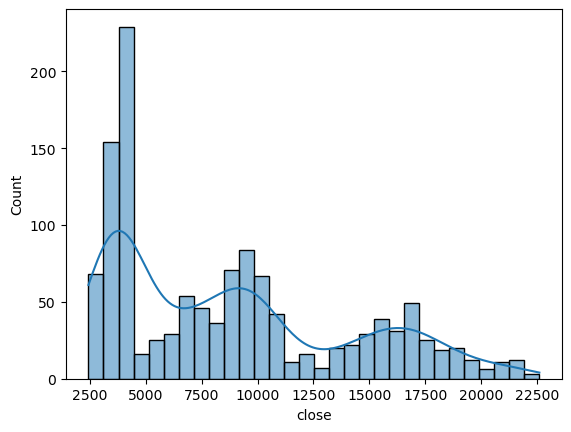
\includegraphics[width=1\textwidth]{bibliography/Figure/elc_hist.png}
    \caption{ELC stock price's histogram}
    \label{fig:2}
    \end{minipage}
\end{figure}

\begin{figure}[H]
    \centering
    \begin{minipage}{0.23\textwidth}
    \centering
    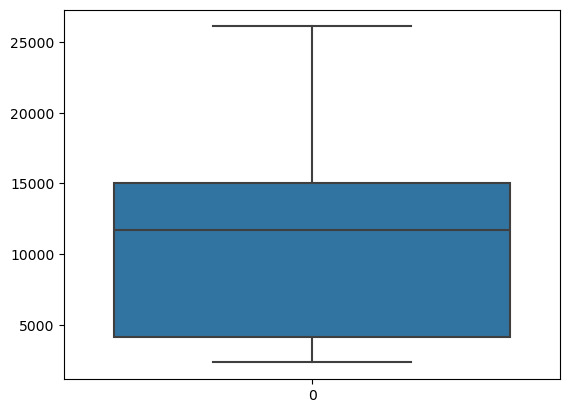
\includegraphics[width=1\textwidth]{bibliography/Figure/sgt_boxplot.png}
    \caption{SGT stock price's boxplot}
    \label{fig:1}
    \end{minipage}
    \hfill
    \begin{minipage}{0.23\textwidth}
    \centering
    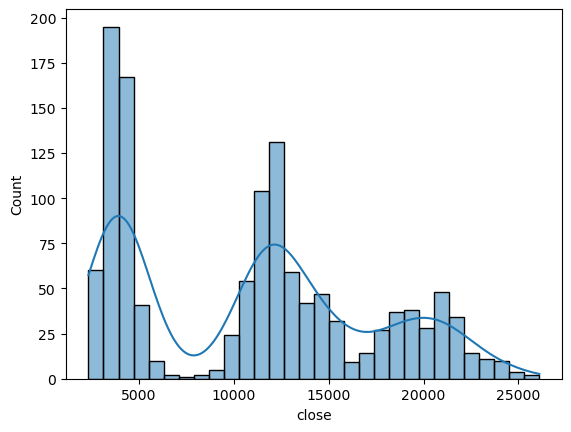
\includegraphics[width=1\textwidth]{bibliography/Figure/sgt_hist.png}
    \caption{SGT stock price's histogram}
    \label{fig:2}
    \end{minipage}
\end{figure}

\section{Methodology}
\subsection{Linear Regression}
Regression analysis is a statistical method used to create mathematical models that describe the relationship between a dependent variable and one or more independent variables. These variables are typically numerical. The goal is to find an equation that can predict the value of the dependent variable based on the values of the independent variables. In a multiple linear regression model, the equation takes the form of:

Dependent Variable = Intercept + Coefficient 1 * Independent Variable 1 + Coefficient 2 * Independent Variable 2 + ... + Coefficient n * Independent Variable n + Error Term

In this equation:

The dependent variable is the variable we want to predict or explain.
The independent variables are the variables that we believe influence or explain the dependent variable.
The intercept term represents the starting point of the regression line.
The regression coefficients (β) represent the impact of each independent variable on the dependent variable.
The error term accounts for the variability or unpredictability of the dependent variable that is not explained by the independent variables.
 
\subsection{ARIMA}
ARIMA model is a generalized model of Autoregressive
Moving Average (ARMA) that combines Autoregressive
(AR) process and Moving Average (MA) processes and
builds a composite model of the time series. [9]
The ARIMA model has three parameters: p, d, q
As the acronym indicates, ARIMA(p, d, q) captures the key
elements of the model [2]: \\
- AR: Autoregression. A regression model that uses the
dependencies between an observation and a number of
lagged observations (p). \\
- I: Integrated. To make the time series stationary by
measuring the differences of observations at different
time (d). \\
- MA: Moving Average. An approach that takes into
accounts the dependency between observations and the
residual error terms when a moving average model is
used to the lagged observations (q). \\
A simple form of an AR model of order p, i.e., AR (p), can
be written as a linear process given by: \\
$$
x_t=c+\sum_{i=1}^p \emptyset_i x_{t-i}+\varepsilon_t
$$
\\
Where $\chi_t$ is the stationary variable, c is constant, the terms in $\emptyset_i$ are autocorrelation coefficients at lags 1, 2, …, $p$ and $\varepsilon_t$ the residuals, are the Gaussian white noise series with mean zero and variance $\sigma_{\varepsilon}^2$ \\ 
An MA model of order q, i.e., MA(q), can be written in the form:
$$
x_t=\mu+\sum_{i=0}^q \theta_i \varepsilon_{t-i}
$$
Where $\mu$ is the expectation of $\chi_t$ (usually assumed equal to zero), the $\emptyset_i$ terms are the weights applied to the current and
prior values of a stochastic term in the time series, and $\theta_0=1$. We assume that $\chi_t$ is a Gaussian white noise series with
mean zero and variance $\sigma_{\varepsilon}^2$. \\ 
We can combine these two models by adding them together
and form an ARMA model of order (p, q):
$$
x_t=c +\sum_{i=1}^p \emptyset_i x_{t-i}+\varepsilon_t + \sum_{i=0}^q \theta_i \varepsilon_{t-i}
$$
Where $\emptyset_i \neq 0$, $\theta_i \neq 0$ and  $\sigma_{\varepsilon}^2 > 0$. The parameters p and q are
called the AR and MA orders, respectively. ARIMA
forecasting, also known as Box and Jenkins forecasting, is
capable of dealing with non-stationary time series data
because of its “integrate” step. \\
In fact, the “integrate” component involves differencing the
time series to convert a non-stationary time series into a
stationary one. The general form of an ARIMA model is denoted
as ARIMA(p, d, q). [2] \\
Applying the ARIMA algorithm to the PVS dataset:
ARIMA (7-2-1) \\








\subsection{ETS (Error, Trend, Seasonal model)}
Exponential smoothing was proposed in the late 1950s (Brown, 1959; Holt, 1957; Winters, 1960), and has motivated some of the most successful forecasting methods. Forecasts produced using exponential smoothing methods are weighted averages of past observations, with the weights decaying exponentially as the observations get older. In other words, the more recent the observation the higher the associated weight. This framework generates reliable forecasts quickly and for a wide range of time series, which is a great advantage and of major importance to applications in industry. 
\subsubsection{ETS(A,N,N): Simple exponential smoothing with additive errors} \
The component form of simple exponential smoothing:\
\begin{center}

    $\hat{y}_{t+1|t} = \ell_t$ \\
    $\ell_t = \alpha y_t + (1 - \alpha)\ell_{t-1} $\\
\end{center}
\subsubsection{ETS(M,N,N): Simple exponential smoothing with multiplicative errors} \
Similarly, we can specify models with multiplicative errors by writing the one-step ahead training errors as relative errors
$$
\varepsilon_t=\frac{y_t-\hat{y}_{t \mid t-1}}{\hat{y}_{t \mid t-1}}
$$
where $\varepsilon_t \sim \operatorname{NID}\left(0, \sigma^2\right)$. Substituting $\hat{y}_{t \mid t-1}=\ell_{t-1}$ gives $y_t=\ell_{t-1}+\ell_{t-1} \varepsilon_t$ and $e_t=y_t-\hat{y}_{t \mid t-1}=\ell_{t-1} \varepsilon_t$.

Then we can write the multiplicative form of the state space model as
$$
\begin{aligned}
& y_t=\ell_{t-1}\left(1+\varepsilon_t\right) \\
& \ell_t=\ell_{t-1}\left(1+\alpha \varepsilon_t\right)
\end{aligned}
$$
\subsubsection{ETS(A,A,N): Holt’s linear method with additive errors} \
For this model, we assume that the one-step-ahead training errors are given by $\varepsilon_t=y_t-\ell_{t-1}-b_{t-1} \sim \operatorname{NID}\left(0, \sigma^2\right)$. Substituting this into the error correction equations for Holt's linear method we obtain
$$
\begin{aligned}
y_t & =\ell_{t-1}+b_{t-1}+\varepsilon_t \\
\ell_t & =\ell_{t-1}+b_{t-1}+\alpha \varepsilon_t \\
b_t & =b_{t-1}+\beta \varepsilon_t,
\end{aligned}
$$
where for simplicity we have set $\beta=\alpha \beta^*$.
\subsubsection{ETS(M,A,N): Holt’s linear method with multiplicative errors} \
Specifying one-step-ahead training errors as relative errors such that
$$
\varepsilon_t=\frac{y_t-\left(\ell_{t-1}+b_{t-1}\right)}{\left(\ell_{t-1}+b_{t-1}\right)}
$$
and following an approach similar to that used above, the innovations state space model underlying Holt's linear method with multiplicative errors is specified as
$$
\begin{aligned}
& y_t=\left(\ell_{t-1}+b_{t-1}\right)\left(1+\varepsilon_t\right) \\
& \ell_t=\left(\ell_{t-1}+b_{t-1}\right)\left(1+\alpha \varepsilon_t\right) \\
& b_t=b_{t-1}+\beta\left(\ell_{t-1}+b_{t-1}\right) \varepsilon_t,
\end{aligned}
$$
where again $\beta=\alpha \beta^*$ and $\varepsilon_t \sim \operatorname{NID}\left(0, \sigma^2\right)$.

\subsection{RNN (Recurrent Neural Network)}
Recurrent Neural Networks (RNNs) are a class of neural networks that are designed to process sequential data, such as text, speech, or time-series data. Unlike traditional feedforward neural networks, which process inputs independently, RNNs maintain an internal state (called the hidden state) that allows them to incorporate information from previous inputs into the current output.

The key idea behind RNNs is that they use the same set of weights (parameters) to process each element of the sequence, with the hidden state being passed from one time step to the next. This allows the network to capture temporal dependencies in the data, which is particularly important for tasks like language modeling, machine translation, and speech recognition.
$$
\begin{aligned}
	h_t &= f(W_x \cdot x_t + W_h \cdot h_{(t-1)} + b) \\
	y_t &= g(W_y \cdot h_t + c)
\end{aligned}
$$
where:
\begin{itemize}
	\item $h_t$ is the hidden state at time $t$
	\item $x_t$ is the input at time $t$
	\item $W_x$, $W_h$, $W_y$ are the weight matrices
	\item $b$, $c$ are the biases
	\item $f$ is a nonlinear activation function, such as $\tanh$ or $\text{ReLU}$
	\item $g$ is the output function, such as a softmax for classification or a linear function for regression
\end{itemize}

The key idea behind RNNs is that they use the same set of weights to process each element of the sequence, with the hidden state being passed from one time step to the next. This allows the network to capture temporal dependencies in the data.

\subsection{LSTM (Long Short-Term Memory)}
Long Short-Term Memory (LSTMs) are an advanced RNN architecture designed to address the vanishing gradient problem. LSTMs introduce specialized gates (forget, input, and output) that control the flow of information into and out of the cell state, allowing the network to store and access information over longer periods of time.

The key components of an LSTM are:
\begin{itemize}
	\item Forget gate ($f_t$): Decides what information from the previous cell state ($C_{t-1}$) to keep or forget.
	\item Input gate ($i_t$): Decides what new information from the current input ($x_t$) and previous hidden state ($h_{t-1}$) to add to the cell state.
	\item Cell state ($C_t$): The "memory" of the LSTM, which is updated based on the forget and input gates.
	\item Output gate ($o_t$): Decides what information from the current cell state ($C_t$) and input ($x_t$) to use to produce the current hidden state ($h_t$).
\end{itemize}

The ability of LSTMs to selectively remember and forget information, as well as their capacity to capture long-term dependencies, has made them a widely used and successful architecture for various sequence-to-sequence tasks.
$$
\begin{aligned}
	f_t &= \sigma(W_f \cdot [h_{t-1}, x_t] + b_f) \\
	i_t &= \sigma(W_i \cdot [h_{t-1}, x_t] + b_i) \\
	\tilde{C}_t &= \tanh(W_C \cdot [h_{t-1}, x_t] + b_C) \\
	C_t &= f_t \odot C_{t-1} + i_t \odot \tilde{C}_t \\
	o_t &= \sigma(W_o \cdot [h_{t-1}, x_t] + b_o) \\
	h_t &= o_t \odot \tanh(C_t)
\end{aligned}
$$
\subsection{GRU (Gated Recurrent Unit)}

Gated Recurrent Unit (GRU) is another type of advanced Recurrent Neural Network (RNN) architecture, similar to Long Short-Term Memory (LSTM) networks. GRUs were introduced as a simpler alternative to LSTMs, aiming to achieve similar performance while reducing the number of parameters and the overall complexity of the model.

The key components of a GRU cell are:

The update gate determines what information from the previous hidden state ($h_{t-1}$) and the current input ($x_t$) should be used to update the current hidden state ($h_t$). The update gate is defined as:
$$
\begin{aligned}
	z_t = \sigma(W_z \cdot [h_{t-1}, x_t] + b_z)
\end{aligned}
$$
where $\sigma$ is the sigmoid activation function, $W_z$ is the weight matrix, and $b_z$ is the bias.

The reset gate decides what information from the previous hidden state ($h_{t-1}$) should be used to compute the current candidate hidden state ($\tilde{h}_t$). This allows the GRU to selectively forget or reset the hidden state based on the current input. The reset gate is defined as:
$$
\begin{aligned}
	r_t = \sigma(W_r \cdot [h_{t-1}, x_t] + b_r)
\end{aligned}
$$

The candidate hidden state is a temporary hidden state that is created based on the current input ($x_t$) and the previous hidden state ($h_{t-1}$) scaled by the reset gate ($r_t$). This candidate state is then used to update the actual hidden state. The candidate hidden state is defined as:
$$
\begin{aligned}
	\tilde{h}t = \tanh(W_h \cdot [r_t \odot h{t-1}, x_t] + b_h)
\end{aligned}
$$
where $\tanh$ is the hyperbolic tangent activation function, and $\odot$ represents element-wise multiplication.

The final hidden state is computed as a linear interpolation between the previous hidden state ($h_{t-1}$) and the candidate hidden state ($\tilde{h}_t$), with the update gate ($z_t$) controlling the balance between the two:
$$
\begin{aligned}
	h_t = (1 - z_t) \odot h_{t-1} + z_t \odot \tilde{h}_t
\end{aligned}
$$

The GRU architecture, with its simplified structure compared to LSTMs, has shown competitive performance in various sequence-to-sequence tasks, such as language modeling, machine translation, and speech recognition, while often requiring fewer parameters and less computational resources.

\subsection{BAGGING MODELS (Bootstrap Aggregating)}
Introduction to Bagging (Bootstrap Aggregating)
Bagging (Bootstrap Aggregating) is a model training technique based on creating sub-samples of data from the original training dataset using bootstrap sampling technique.

\begin{figure}[H]
    \centering
    \begin{minipage}{0.23\textwidth}
    \centering
    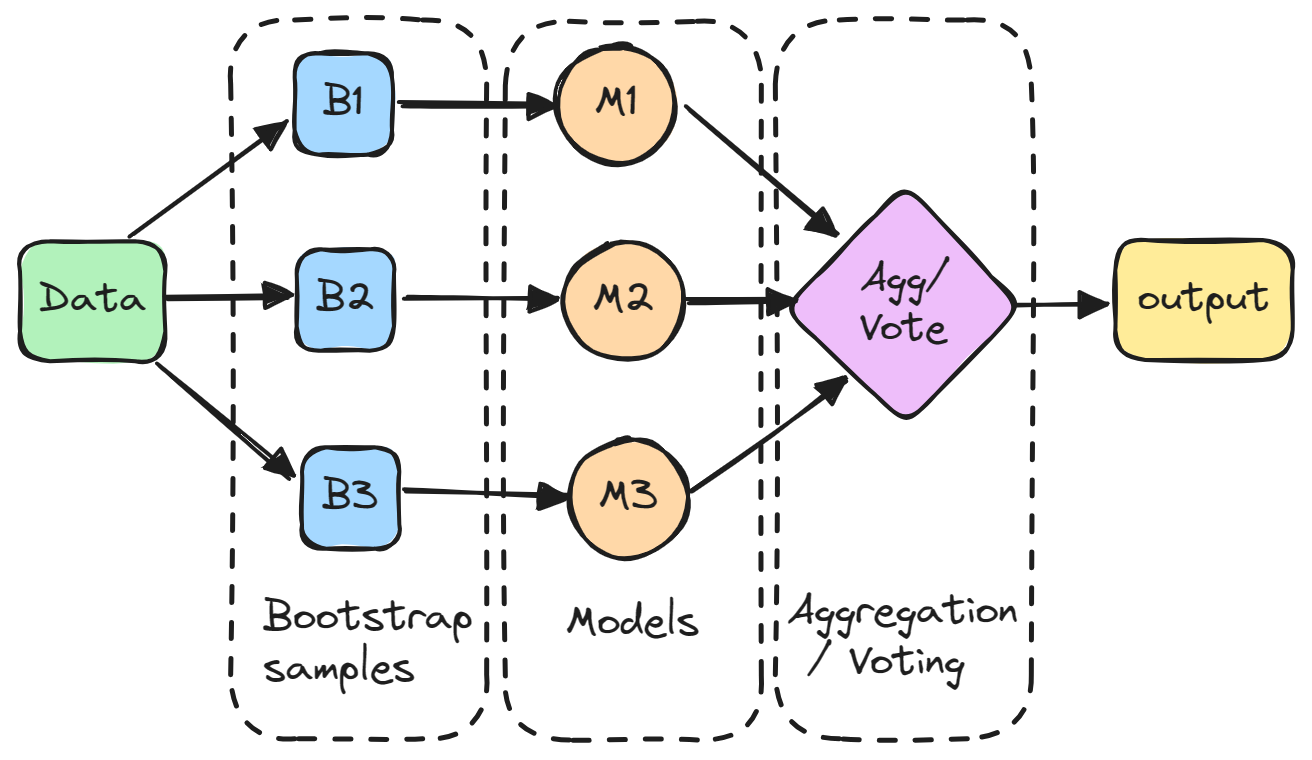
\includegraphics[width=1\textwidth]{bibliography/BG_Describe.png}
    \caption{SGT stock price's boxplot}
    \label{fig:1}
    \end{minipage}
    \hfill
\end{figure}
How Bagging Works:
Bootstrap Sampling: Firstly, a large number of data subsets are created from the original training dataset by randomly sampling with replacement.

Model Training: A base model is trained on each data subset.

Aggregating: The final prediction is computed by combining predictions from all base models. In regression problems, this is often done by averaging predictions from individual models.

Advantages of Bagging:
Variance Reduction: By combining multiple base models, Bagging reduces the variance in predictions, thereby improving the stability and accuracy of the model.

Reduces Overfitting: Bagging helps minimize the phenomenon of overfitting by reducing the sensitivity of the model to specific training data.

Flexibility: Bagging can be applied to various types of machine learning models and requires few hyperparameters.

Applications of Bagging:
Bagging is commonly used in regression and classification problems to enhance the predictive performance of the model.

It can also be applied to reduce noise in datasets with a high level of noise.

Bagging is a powerful and widely-used model training technique in machine learning to improve prediction performance and mitigate overfitting. By combining data from multiple base models, Bagging creates a generalized and robust model suitable for various real-world applications.
\section{Result}
\subsection{Evaluation Methods}
\textbf{Mean Percentage Absolute Error} (MAPE): is the average percentage error in a set of predicted values.\\
\[MAPE=\frac{100\%}{n}  \sum_{i=1}^{n} |y_i-\hat{y_i} |  = 1 \]\\
\textbf{Root Mean Squared Error} (RMSE): is the square root of an average value of squared error in a set of predicted values.\\
\[RMSE=\sqrt{\sum_{i=1}^{n} \frac{(\hat{y_i}-y_i )^2}{n} }\]\\
\textbf{Mean Absolute Error} (MSLE): is the relative difference between the log-transformed actual and predicted values.\\
\[MSLE=\frac{1}{n}\sum_{i=1}^{n}(log(1+\hat{y_i})-log(log(1+y_i))^2\]
Where: \\
	\indent\textbullet\ \(n\) is the number of observations in the dataset.\\
	\indent\textbullet\ \(y_i\)  is the true value.\\
	\indent\textbullet\ \(\hat{y_i}\) is the predicted value.
\subsection{ELC Dataset} 
\begin{table}[H]
    \centering
    \begin{tabular}{|c|c|c|c|c|}
         \hline
         \multicolumn{5}{|c|}{\textbf{ELC Dataset's Evaluation}}\\
         \hline
         \centering Model & Training:Testing & RMSE & MAPE (\%) & MSLE\\
         \hline
         \multirow{2}{*}{LN} & 7:3 & 5711.84 & 57.59 &0.257 \\ & \textbf{8:2} & \textbf{3894.03} & \textbf{25.91} & \textbf{0.072} \\ & 9:1 & 5561.64 & 27.88 & \textbf0.116\\
         \hline
         \multirow{2}{*}{ARIMA} & 7:3 &  5839.19&  29.78 & 0.2 \\ & 8:2 &  7063.12 & 31.1 & 0.27 \\ & \textbf{9:1} & \textbf{2166.68}  & \textbf{9.14} & \textbf{0.013}\\
         \hline
         \multirow{2}{*}{ETS} & 7:3 & 9181.45 & 49.74 & 0.99 \\ & 8:2  &   8345.00 &41.94 & 0.48 \\ & \textbf{9:1} &  	\textbf{5540.29} &	\textbf{25.48} & 	\textbf{0.062} \\
         \hline
         \multirow{2}{*}{BAGGING} & \textbf{7:3} & \textbf{8308.33} & \textbf{125.61} & \textbf{0.77} \\ & 8:2  &   9324.83 &158.72 & 0.96 \\ & 9:1 &  	11152.89 & 202.26 & 1.23 \\
         \hline
    \end{tabular}
    \caption{ELC Dataset's Evaluation}
    \label{vcbresult}
\end{table}

\begin{figure}[H]
  \centering
  \begin{minipage}{0.8\linewidth}
    \centering
    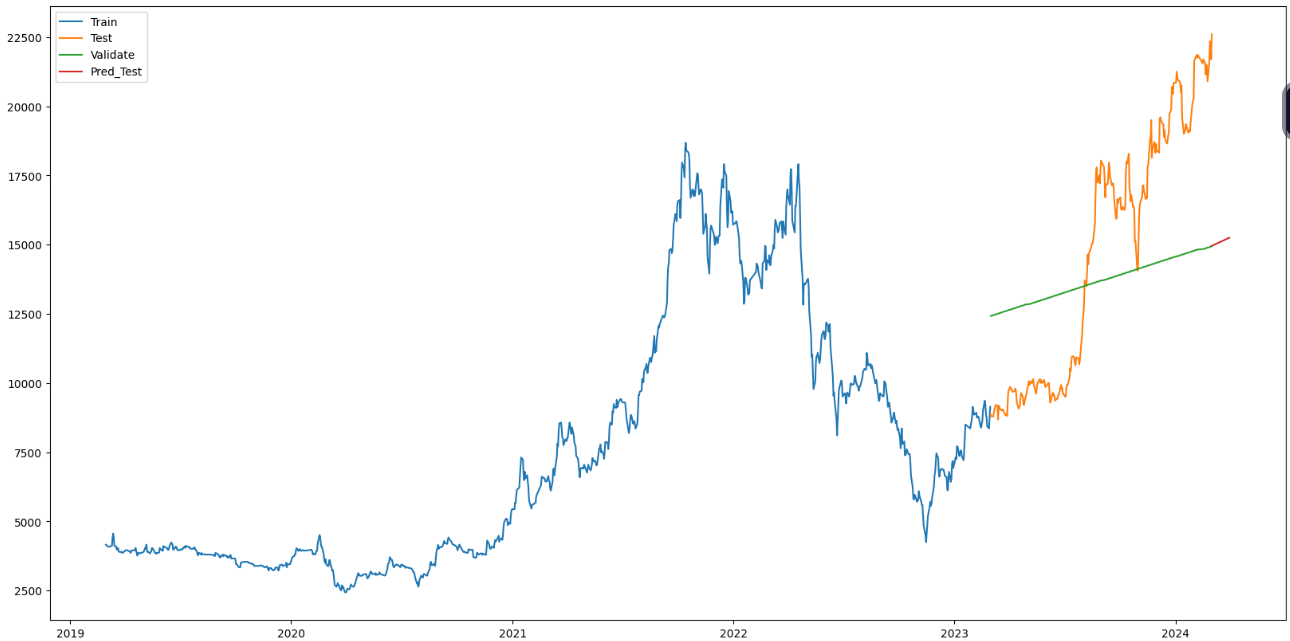
\includegraphics[width=\linewidth]{bibliography/Ln_ELC_82.png}
    \caption{Linear model's result with 8:2 splitting proportion}
    \label{fig8}
  \end{minipage}
\end{figure}
\begin{figure}[H]
  \centering
  \begin{minipage}{0.8\linewidth}
    \centering
    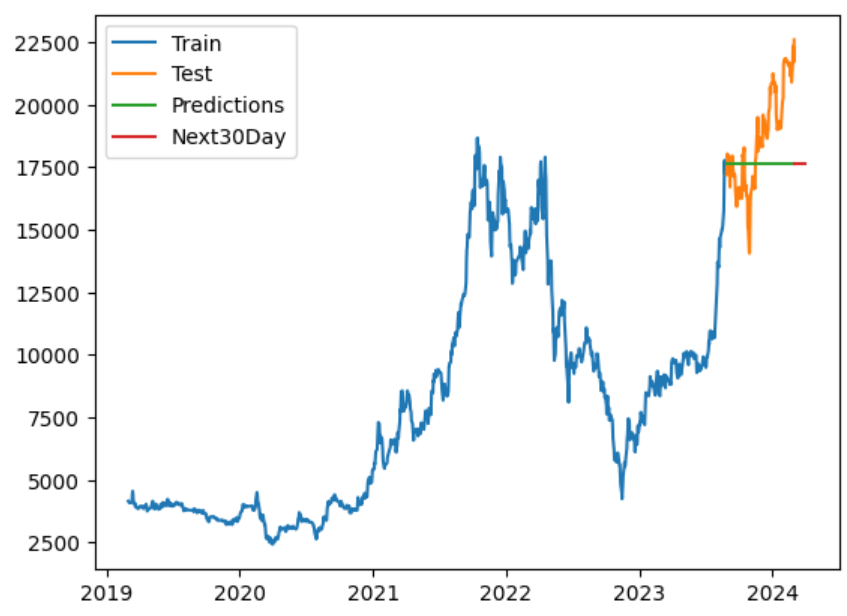
\includegraphics[width=\linewidth]{bibliography/ARIMA_ELC_91.png}
    \caption{ARIMA model's result with 9:1 splitting proportion}
    \label{fig11}
  \end{minipage}
\end{figure}
\begin{figure}[H]
  \centering
  \begin{minipage}{0.8\linewidth}
    \centering
    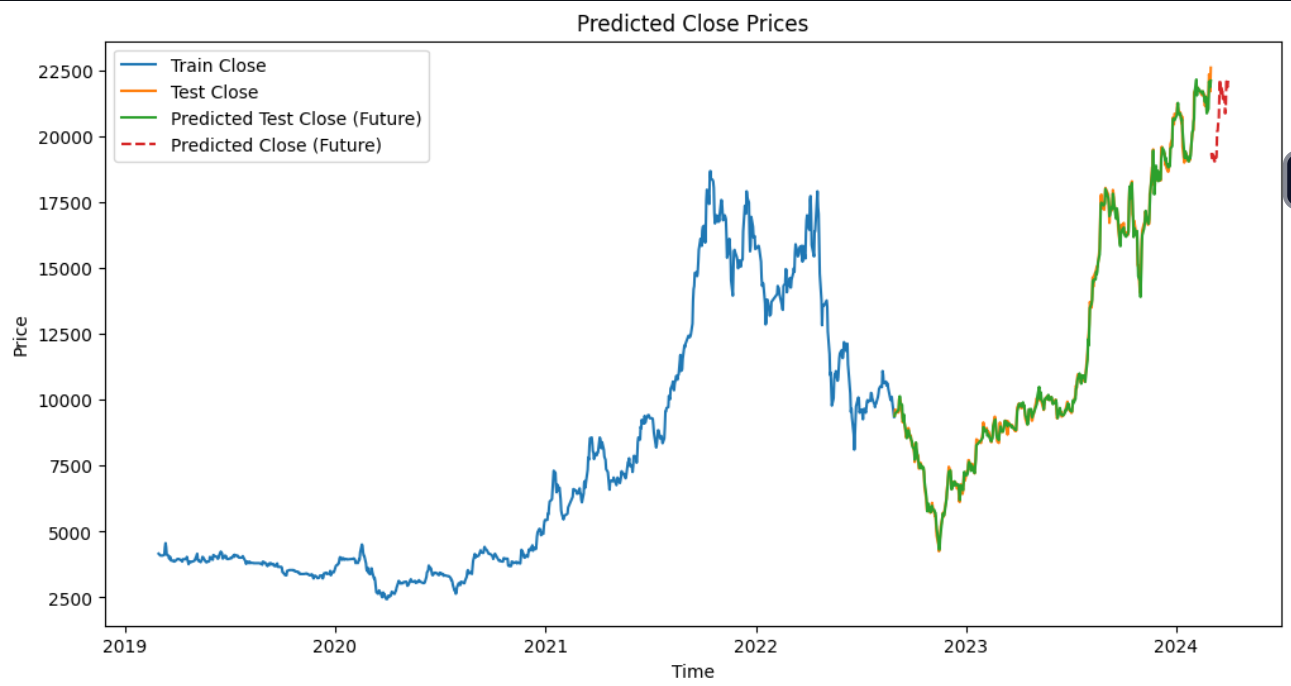
\includegraphics[width=\linewidth]{bibliography/BG_ELC_73.png}
    \caption{ETS model's result with 9:1 splitting proportion}
    \label{fig12}
  \end{minipage}
\end{figure}
\begin{figure}[H]
  \centering
  \begin{minipage}{0.8\linewidth}
    \centering
    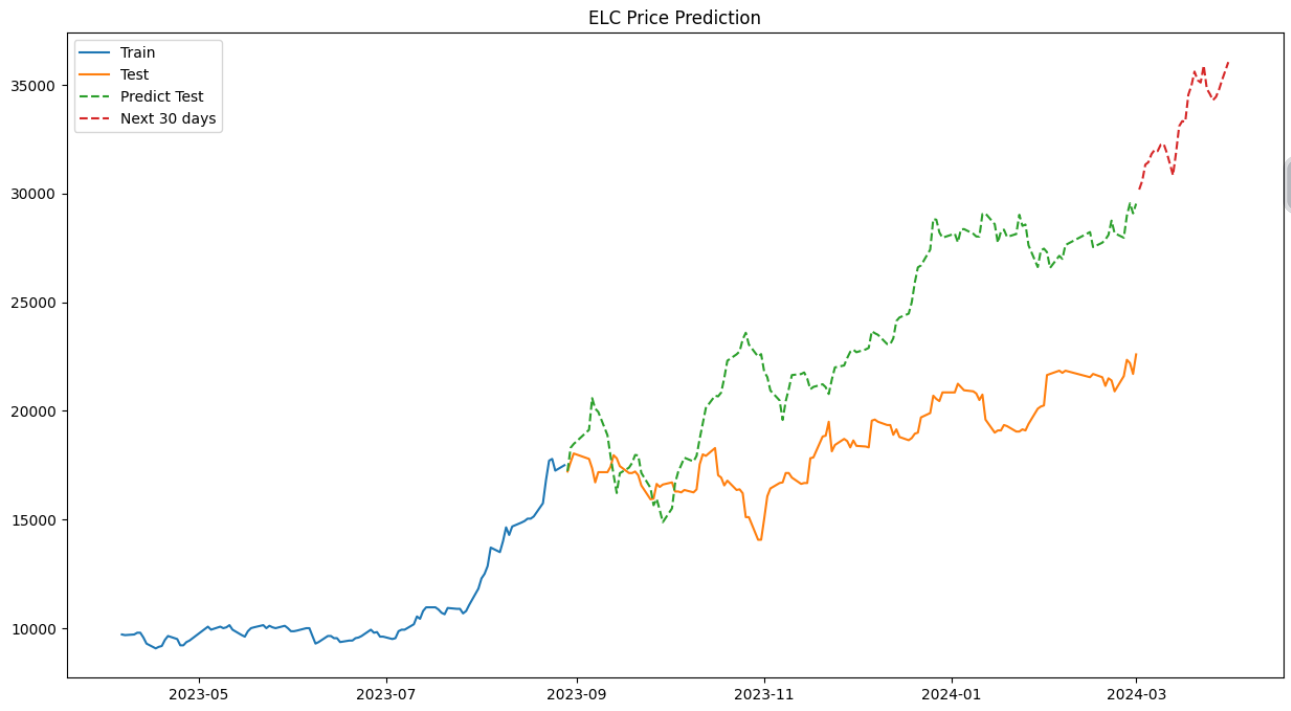
\includegraphics[width=\linewidth]{bibliography/ETS_ELC_91.png}
    \caption{BAGGING(KNN-LINEAR) model's result with 7:3 splitting proportion}
    \label{fig12}
  \end{minipage}
\end{figure}


\subsection{FPT dataset} 
\begin{table}[H]
    \centering
    \begin{tabular}{|c|c|c|c|c|}
         \hline
         \multicolumn{5}{|c|}{\textbf{FPT Dataset's Evaluation}}\\
         \hline
         \centering Model & Training:Testing & RMSE & MAPE (\%) & MSLE\\
         \hline
         \multirow{2}{*}{LN} & 7:3 & 12414.36 & 15.27 & 0.026\\ & \textbf{8:2} & \textbf{8708.75} &\textbf{9.64} & \textbf{0.011} \\ & 9:1 & 10514.15 & 9.91 & 0.012\\
         \hline
         \multirow{2}{*}{ARIMA} & 7:3 &  10889.73 &  13.13 & 0.02 \\ & 8:2 &  12926.62 & 11.09 &  0.02\\ & \textbf{9:1} & \textbf{5004.96} & \textbf{4.64} & \textbf{0.002}\\
         \hline
         \multirow{2}{*}{ETS} & 7:3 & 14500.10 & 13.28 &0.031 \\ & 8:2  & 17608.12 &14.87 & 0.044\\ & \textbf{9:1} &  	\textbf{5556.23} &	\textbf{4.95} & 	\textbf{0.0034} \\
         \hline
          \multirow{2}{*}{BAGGING} & \textbf{7:3} & \textbf{37744.61} & \textbf{93.68} & \textbf{0.51} \\ & 8:2  &   9329.07 &158.77 & 0.96 \\ & 9:1 &  11158.14 &	202.36 & 1.23 \\
         \hline
    \end{tabular}
    \caption{FPT Dataset's Evaluation}
    \label{vcbresult}
\end{table}

\begin{figure}[H]
  \centering
  \begin{minipage}{0.8\linewidth}
    \centering
    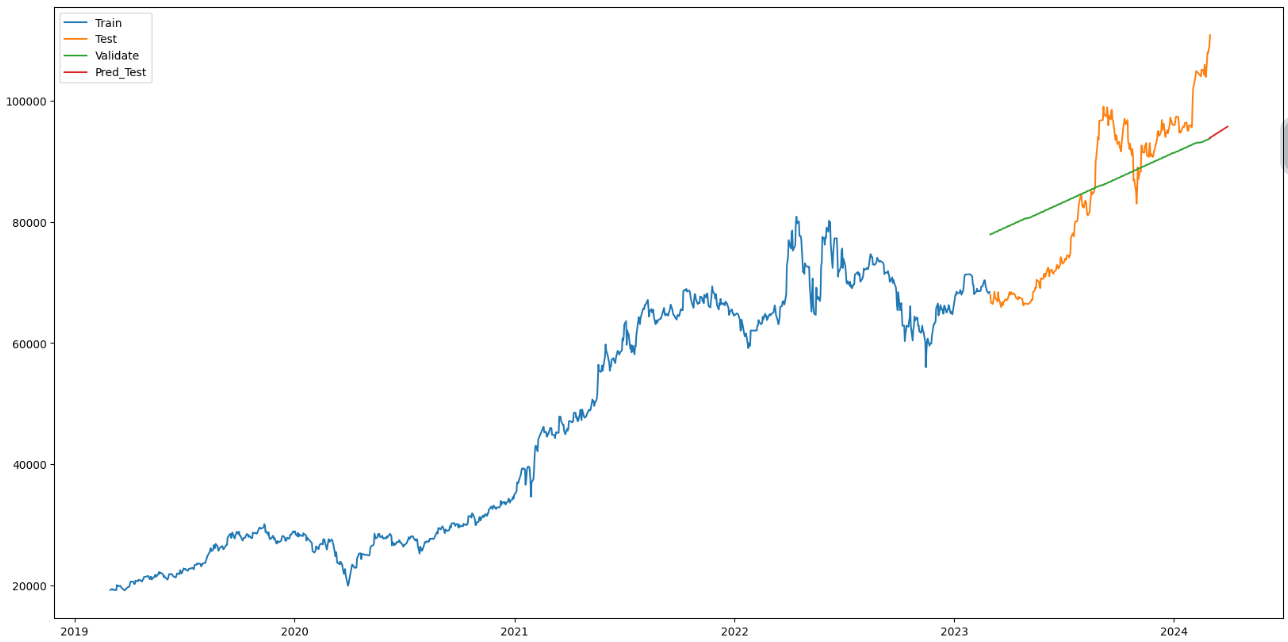
\includegraphics[width=\linewidth]{LN_FPT,82.png}
    \caption{Linear model's result with 8:2 splitting proportion}
    \label{fig15}
  \end{minipage}
\end{figure}
\begin{figure}[H]
  \centering
  \begin{minipage}{0.8\linewidth}
    \centering
    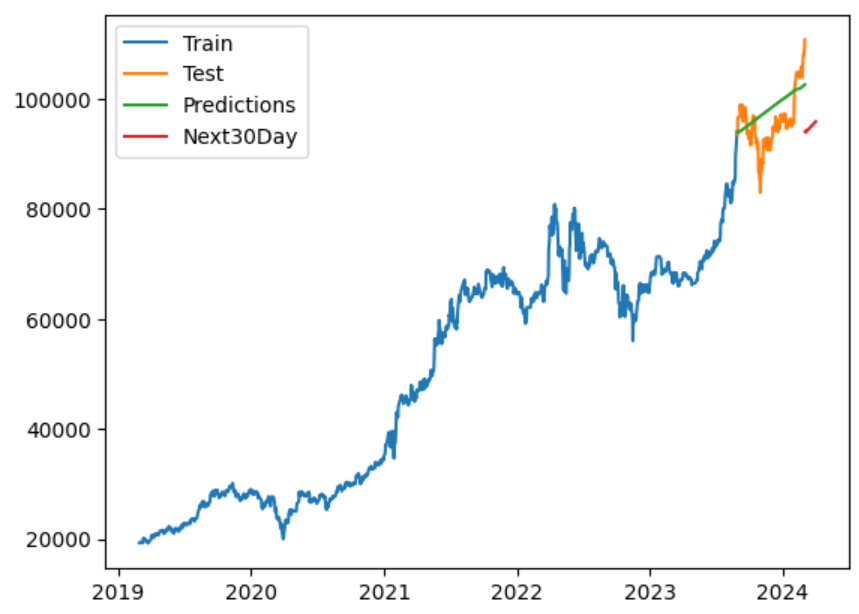
\includegraphics[width=\linewidth]{bibliography/ARIMA_FPT_91.png}
    \caption{ARIMA model's result with 9:1 splitting proportion}
    \label{fig16}
  \end{minipage}
\end{figure}
\begin{figure}[H]
  \centering
  \begin{minipage}{0.8\linewidth}
    \centering
    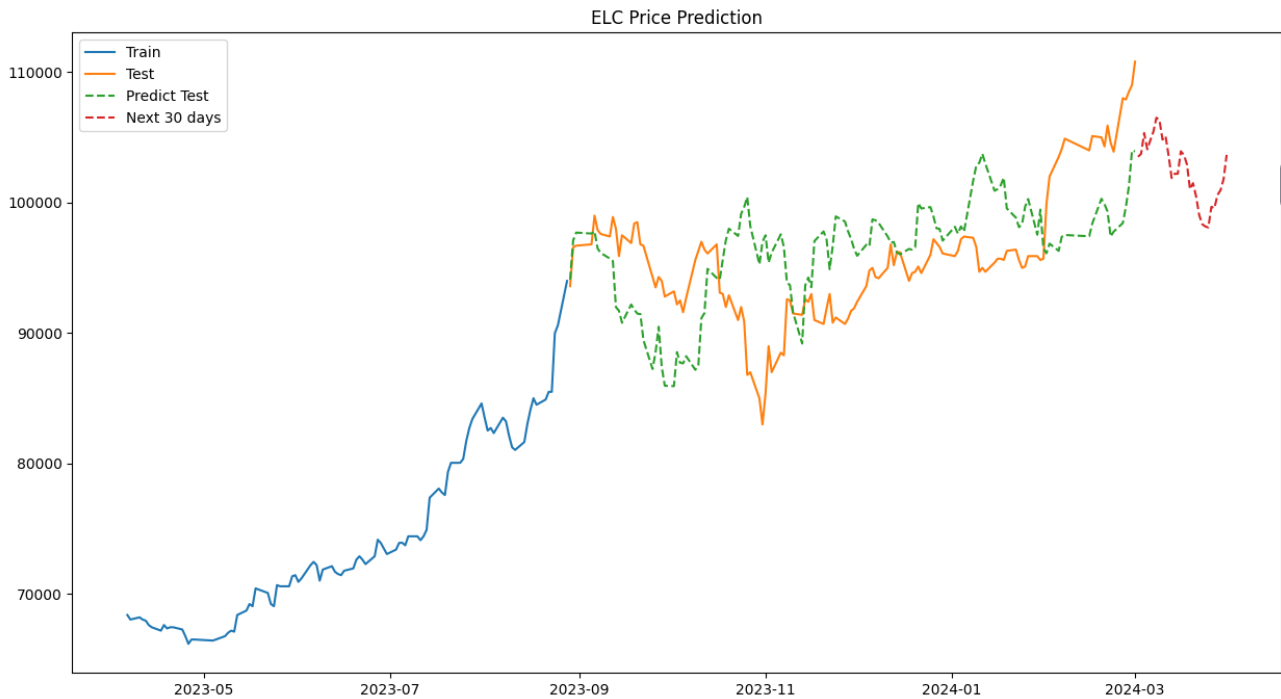
\includegraphics[width=\linewidth]{bibliography/ETS_FPT_91.png}
    \caption{ETS model's result with 9:1 splitting proportion}
    \label{fig17}
  \end{minipage}
\end{figure}
\begin{figure}[H]
  \centering
  \begin{minipage}{0.8\linewidth}
    \centering
    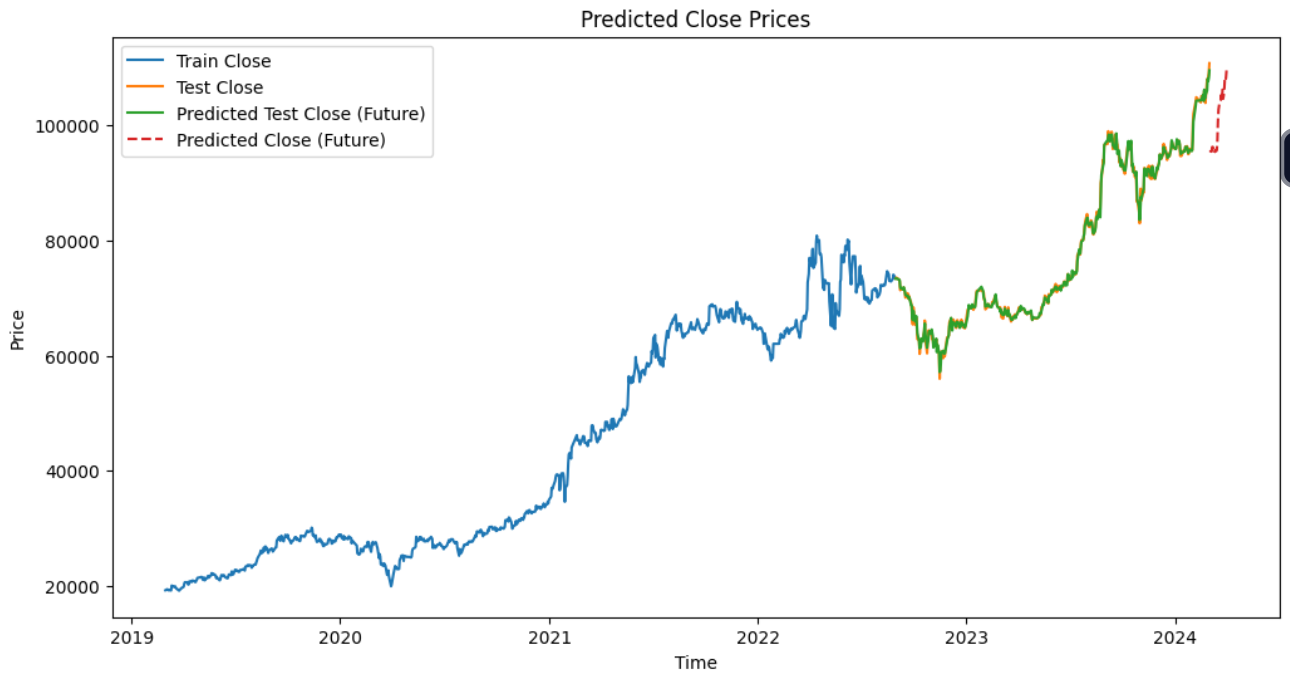
\includegraphics[width=\linewidth]{bibliography/BG_FPT_73.png}
    \caption{BAGGING(KNN-LN) model's result with 7:3 splitting proportion}
    \label{fig17}
  \end{minipage}
\end{figure}




\subsection{SGT dataset} 
\begin{table}[H]
    \centering
    \begin{tabular}{|c|c|c|c|c|}
         \hline
         \multicolumn{5}{|c|}{\textbf{SGT Dataset's Evaluation}}\\
         \hline
         \centering Model & Training:Testing & RMSE & MAPE (\%) & MSLE\\
         \hline
         \multirow{2}{*}{LN} & 7:3 & 13215.73 & 102.30 & 0.50 \\ & 8:2 & 9619.46 & 75.29 & 0.32 \\ & \textbf{9:1} & \textbf{7293.17} & \textbf{57.31} & \textbf{0.21}\\
         \hline
         \multirow{2}{*}{ARIMA} & 7:3 &  5892.15 &  45.82 &0.15 \\ & \textbf{8:2} &  \textbf{1495.67} & \textbf{7.47} & \textbf{0.012} \\ & 9:1 & 2539.03 & 18.83 & 0.035\\
         \hline
         \multirow{2}{*}{ETS} & 7:3 & 5912.57 & 43.018 & 0.145 \\ & \textbf{8:2}  & \textbf{1551.00} &\textbf{10.04} &  \textbf{0.0137} \\ & 9:1 &  	3641.80 &	25.96 & 	0.066 \\
         \hline
          \multirow{2}{*}{BAGGING} & \textbf{7:3} & \textbf{37748.16} & \textbf{93.69} & \textbf{0.51} \\ & 8:2  &   41920.66 &106.36 & 0.60 \\ & 9:1 &  	48563.48 & 127.79 & 0.73 \\
         \hline
    \end{tabular}
    \caption{SGT Dataset's Evaluation}
    \label{vcbresult}
\end{table}

\begin{figure}[H]
  \centering
  \begin{minipage}{0.8\linewidth}
    \centering
    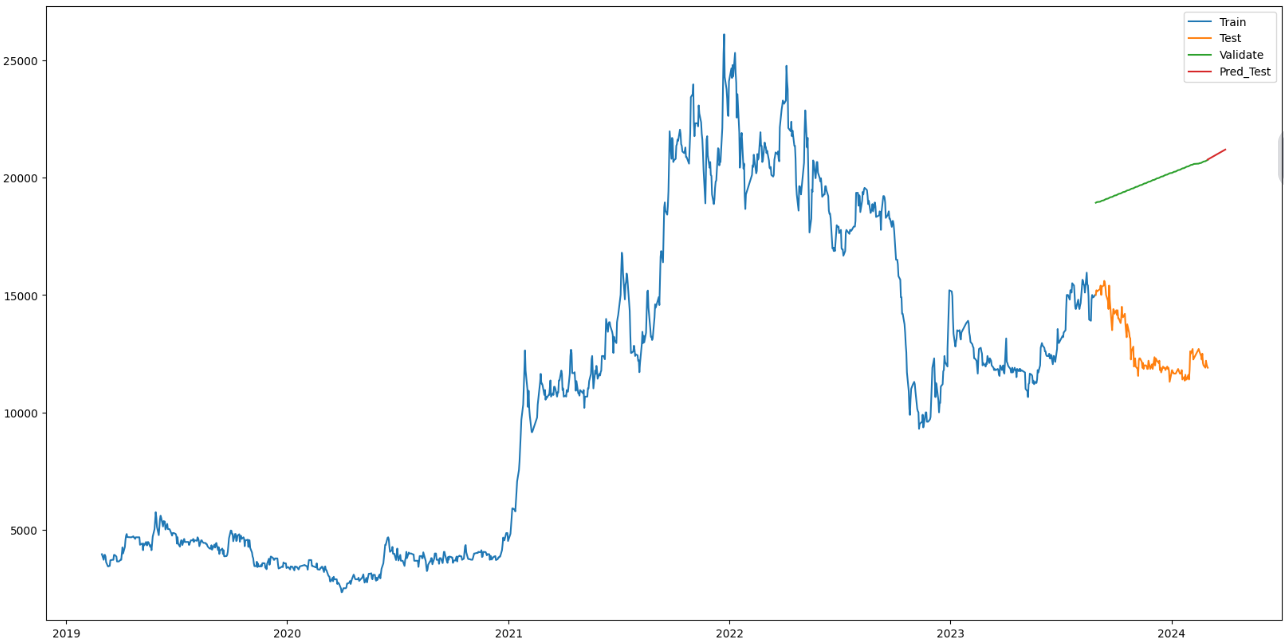
\includegraphics[width=\linewidth]{bibliography/LN_SGT_91.png}
    \caption{Linear model's result with 9:1 splitting proportion}
    \label{fig22}
  \end{minipage}
\end{figure}
\begin{figure}[H]
  \centering
  \begin{minipage}{0.8\linewidth}
    \centering
    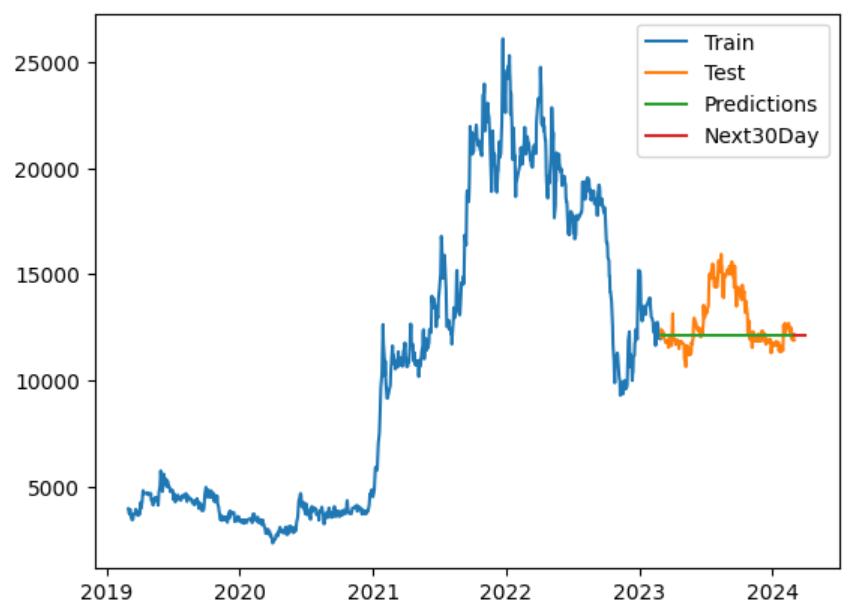
\includegraphics[width=\linewidth]{ARIMA_SGT_82.png}
    \caption{ARIMA model's result with 8:2 splitting proportion}
    \label{fig23}
  \end{minipage}
\end{figure}
\begin{figure}[H]
  \centering
  \begin{minipage}{0.8\linewidth}
    \centering
    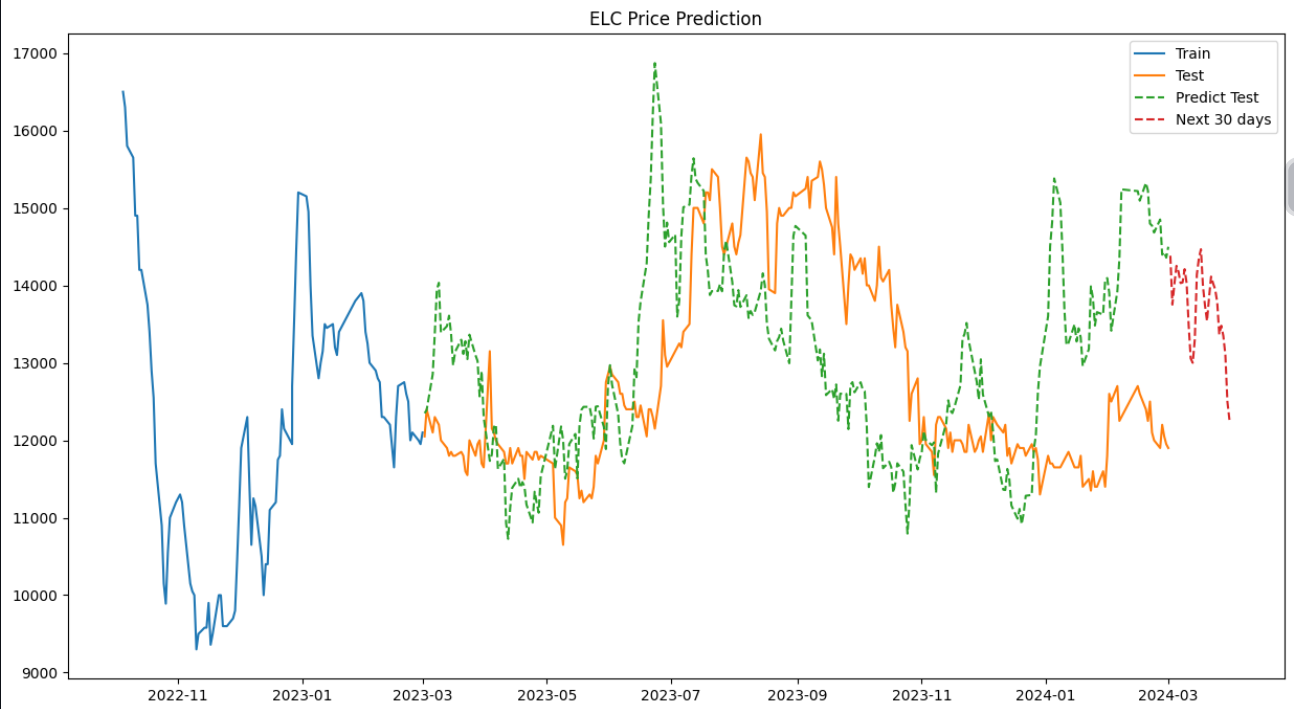
\includegraphics[width=\linewidth]{bibliography/ETS_SGT_82.png}
    \caption{ETS model's result with 8:2 splitting proportion}
    \label{fig24}
  \end{minipage}
\end{figure}
\begin{figure}[H]
  \centering
  \begin{minipage}{0.8\linewidth}
    \centering
    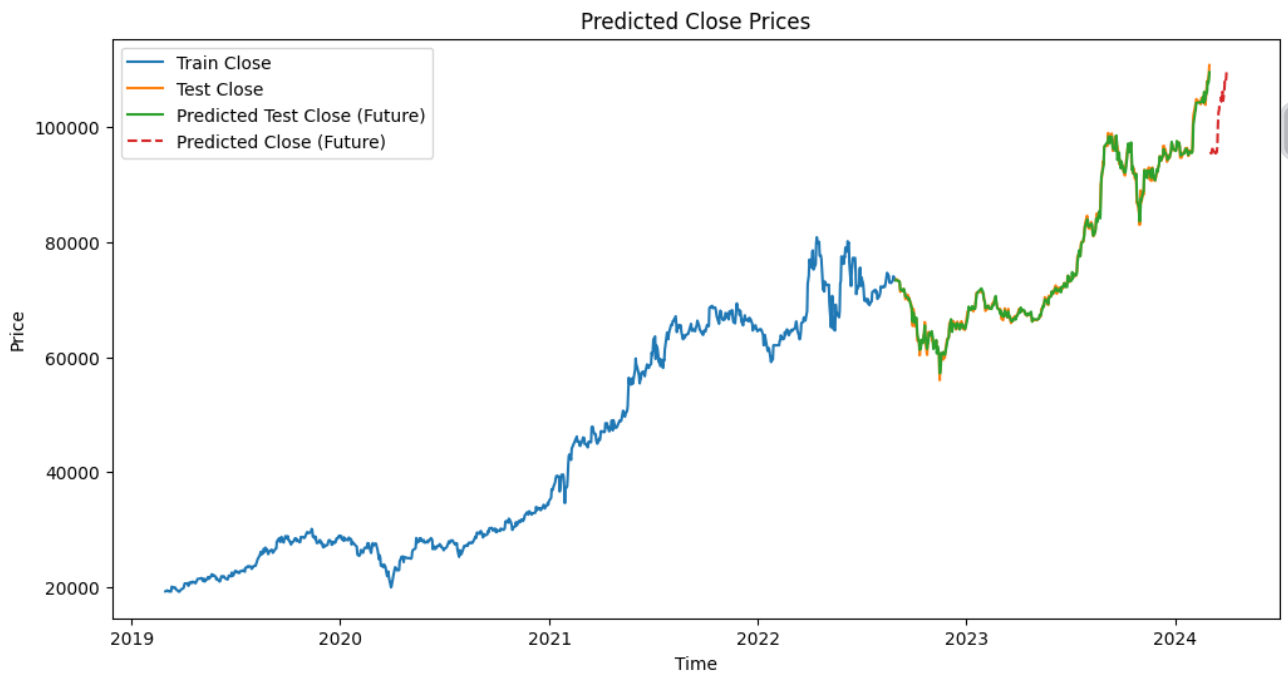
\includegraphics[width=\linewidth]{bibliography/BG_SGT_73.png}
    \caption{ETS model's result with 7:3 splitting proportion}
    \label{fig24}
  \end{minipage}
\end{figure}




\section{Conclusion}
\subsection{Summary}
In the achievement of forecasting stock prices, the exploration of diverse methodologies, ranging from traditional statistical models to advanced machine learning algorithms, has been aimed. Among the performed models, Linear Regression (LR), Auto Regressive Integrated Moving Average (ARIMA), Support Vector Regression (SVR), Seasonal Auto Regression Integrated Moving Average (SARIMA), Dynamic Linear Model (DLM), Bagging – GRU, and Simple Exponential Smoothing (SES), it becomes evident that Support Vector Regression (SVR), Gated Recurrent Unit (GRU), and Bagging GRU emerge as the most promising and effective models for predicting stock prices.\\
The intricacies of stock price forecasting, rooted in the complexity and unpredictability of financial markets, demand models that can capture nuanced patterns and relationships within the data. Support Vector Regression (SVR) showcases its efficacy in handling intricate relationships, providing robust predictions. Gated Recurrent Unit (GRU) models, with their ability to capture sequential dependencies, exhibit notable performance in forecasting stock prices. The introduction of ensemble learning through Bagging GRU further refines the predictive capabilities, offering a collective insight that surpasses individual models.\\
As evidenced by the evaluation metrics, including RMSE, MAPE, and MSLE, the SVR, GRU, and Bagging GRU models consistently demonstrate superior performance across various aspects of forecasting accuracy. Their adaptability to handle the inherent uncertainties of stock markets positions them as formidable tools for investors and analysts seeking reliable predictions.
\subsection{Future Considerations}
In our future research, it is crucial to prioritize further optimization of the previously mentioned models. This optimization effort should specifically focus on:\\
\indent\textbullet\ Enhancing the accuracy of the model. While the above algorithms have demonstrated promising results in predicting stock prices, there is a need to further improve the model's accuracy to ensure more precise forecasting outcomes.\\
\indent\textbullet\ Exploring alternative machine learning algorithms or ensemble techniques. Ensemble techniques, such as combining multiple models or using various ensemble learning methods, can also improve the robustness and accuracy of the forecasts.\\
\indent\textbullet\ Researching new forecasting models. The field of forecasting continuously evolves, with new algorithms and models being researched and developed. It is crucial to stay updated with these approaches and explore new forecasting models that offer improved accuracy and performance. \\
By continuously exploring and incorporating new features, data sources, and modeling techniques, we can strive for ongoing optimization of the forecasting models and enhance their ability to predict stock prices with greater precision and reliability.
\section*{Acknowledgment}
\addcontentsline{toc}{section}{Acknowledgment}
First and foremost, we would like to express our sincere gratitude to \textbf{Assoc. Prof. Dr. Nguyen Dinh Thuan} and \textbf{Mr. Nguyen Minh Nhut} for their exceptional guidance, expertise, and invaluable feedback throughout the research process. Their mentorship and unwavering support have been instrumental in shaping the direction and quality of this study. Their profound knowledge, critical insights, and attention to detail have significantly contributed to the success of this research.
\\This research would not have been possible without the support and contributions of our mentors. We would like to extend our heartfelt thanks to everyone involved for their invaluable assistance, encouragement, and belief in our research. Thank you all for your invaluable assistance and encouragement.

%% UNCOMMENT these lines below (and remove the 2 commands above) if you want to embed the bibliografy.
\begin{thebibliography}{00}
\bibitem{b1} V. Gururaj,  ''Stock Market Prediction using Linear Regression and Support Vector Machines'' vol. 14, no. 8, 2019.
\bibitem{b2} YURTSEVER, M., 2021. Gold price forecasting using LSTM, Bi-LSTM and GRU. Avrupa Bilim ve Teknoloji Dergisi, (31), pp.341-347.
\bibitem{b3} Kishanna, H., RamaParvathyb, L. and SIMATS, C., 2022. A Novel Approach for Correlation Analysis on FBProphet to Forecast Market Gold Rates with Linear Regression.
\bibitem{b4} A. O. A. A. A. Ariyo, ``Stock Price Prediction Using the ARIMA Model'' ,2014. [Online]. Available:https://ieeexplore.ieee.org/document/7046047..
\bibitem{b5} M. S. S. S. A. F. K. Senthamarai Kannan, ``Comparison Of Fuzzy Time Series And ARIMA''August 2019. [Online]. Available:https://www.ijstr.org/final-print/aug2019/Comparison-Of-Fuzzy-Time-Series-And-Arima-Model.pdf. [Accessed 19 June 2023].
\bibitem{b6} B. M. Henrique, V. A. Sobrero, and H. Kimura, ''Stock price prediction using support vector regression on daily and up to the minute prices'' J. Finance Data Sci., vol. 4,no. 3, pp. 183–201, Sep. 2018, doi: 10.1016/j.jfds.2018.04.003. 5
\bibitem{b7}Avner Abrami, Aleksandr Y. Aravkin, Younghun Kim, ''Time Series Using Exponential Smoothing Cells'', 9 June 2017.
\bibitem{b8}  Professor Thomas B. Fomby, ''Exponential Smoothing Models'', June 2008.
\bibitem{b9} Bauer, E., Kohavi, R. ''An Empirical Comparison of Voting Classification Algorithms: Bagging, Boosting, and Variants''. Machine Learning 36, 105–139 (1999). https://doi.org/10.1023/A:1007515423169.
\bibitem{b10} Buja, A., and Stuetzle, W. ''Observations on bagging''. University of Pennsylvania and University of Washington, Seattle. 2002.
\bibitem{b11} B. M. Henrique, V. A. Sobrero, and H. Kimura, ``Comparison Of Fuzzy Time Series And ARIMA'', August 2019. Available:https://www.ijstr.org/final-print/aug2019/Comparison-Of-Fuzzy-Time-Series-And-Arima-Model.pdf. [Accessed 19 June 2023]. 4
\bibitem{b12} Jason Brownlee, ``How to Create an ARIMA Model for Time Series Forecasting in Python'', November 18, 2023. Available:https://www.ijstr.org/final-print/aug2019/Comparison-Of-Fuzzy-Time-Series-And-Arima-Model.pdf. 
\bibitem{b13} Jason Brownlee, ``A Gentle Introduction to SARIMA for Time Series Forecasting in Python'', August 21, 2019. 
\bibitem{b14} Alexandra M. Schmidt and Hedibert F. Lopes, ''Dynamic models'', 2019. 
\bibitem{b15} Timothy O. Hodson, ''Root-mean-square error (RMSE) or mean absolute error (MAE): when to use them or not'', 2022, https://doi.org/10.5194/gmd-15-5481-2022.
\bibitem{b16} Priya Pedamkar,''Support Vector Regression'', March 24, 2023. Retrieved from \(https://www.educba.com/support-vector-regression/?fbclid=IwAR0ibzdmqpaaDKq2-Q4JRcjxQcVt-C7TrHNEc90q_tCSrn8rds9x2AG8Y78\)
\bibitem{b17} Seok-Ho Han, Husna Mutahira, Hoon-Seok Jang, "Prediction of Sensor Data in a Greenhouse for Cultivation of Paprika Plants Using a Stacking Ensemble for Smart Farms", Applied Sciences, vol.13, no.18, pp.10464, 2023.

\end{thebibliography}
%%%%%%%%%%%%%%%


\EOD

\end{document}
